\documentclass[conference]{IEEEtran}
\IEEEoverridecommandlockouts
% The preceding line is only needed to identify funding in the first footnote. If that is unneeded, please comment it out.
\usepackage{cite}
\usepackage{amsmath,amssymb,amsfonts}
\usepackage{algorithmic}
\usepackage{graphicx}
\usepackage{textcomp}
\usepackage{xcolor}
\def\BibTeX{{\rm B\kern-.05em{\sc i\kern-.025em b}\kern-.08em
		T\kern-.1667em\lower.7ex\hbox{E}\kern-.125emX}}
\begin{document}
	
	\title{Report 8}
	
	\author{\IEEEauthorblockN{1\textsuperscript{st} Ali Ramezanzadeh}
		\IEEEauthorblockA{\textit{dept. of Electrical Engineering} \\
			\textit{Amirkabir University of Technology}\\
			Tehran, Iran\\
			ali.ramezan@aut.ac.ir}
		\and
		\IEEEauthorblockN{2\textsuperscript{nd} Arian Abdollahi}
		\IEEEauthorblockA{\textit{dept. of Electrical Engineering} \\
			\textit{Amirkabir University of Technology}\\
			Tehran, Iran\\
			arian.abdollahi@aut.ac.ir}
		\and
		\IEEEauthorblockN{3\textsuperscript{rd} Sina Shah Mohammadi}
		\IEEEauthorblockA{\textit{dept. of Electrical Engineering} \\
			\textit{Amirkabir University of Technology}\\
			Tehran, Iran\\
			alisinashahmohammadi@aut.ac.ir}}
	
	\maketitle

	
	\section{Introduction}
In this experiment, we want to design a lead and lag controller for an flexible joint robot.\newline
A flexible joint robot is a type of robot designed with joints that offer some degree of flexibility, compliance, or elasticity, distinguishing them from rigid robots. These robots incorporate elements like springs, elastic actuators, or specially designed mechanisms to allow controlled movement with some give or deformation at the joints. 

	\begin{figure}[htbp]
	\centerline{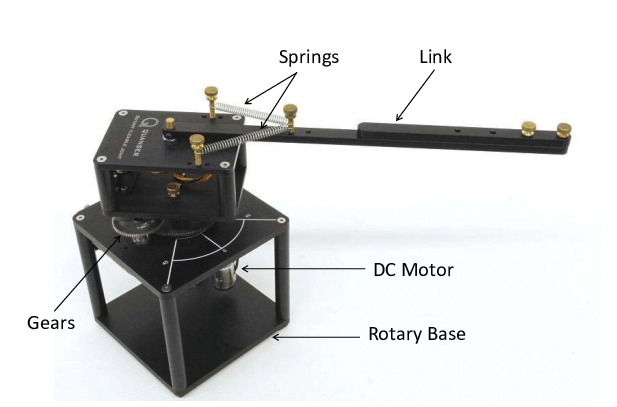
\includegraphics[width=0.7\linewidth]{1.jpg}}
	\caption{Flexible Joint Robot}
	\label{fig1}
\end{figure}

	\section{Mathematical Modeling}
We use the following diagram to derive the mathematical model of the system:

\begin{figure}[htbp]
	\centerline{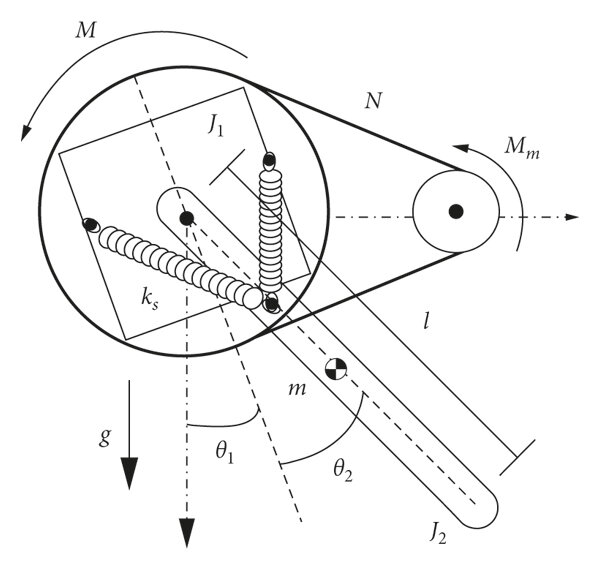
\includegraphics[width=0.7\linewidth]{2.jpg}}
	\caption{Flexible Joint Robot Model}
	\label{fig2}
\end{figure}

Using Lagrange-Hamilton, we arrive at the following equations.


\begin{equation}
	J_{eq} \ddot{\theta}+ J_{Arm}( \ddot{\theta}+\ddot{\alpha})=T_{output}-B_{eq}\dot{\theta}
\end{equation}


\begin{equation}
J_{Arm}( \ddot{\theta}+\ddot{\alpha})+K_{stiff}\alpha=0
\end{equation}

And we have the torque of a DC motor:

\begin{equation}
	T_{output}=\dfrac{\eta_{m}\eta_{g}K_{g}K_{m}(V_{m}-K_{g}K_{m}\dot{\theta})}{R_{m}}
\end{equation}
The selected state variables are:

\[
X=
\begin{pmatrix}
	\theta \\
	\dot{\theta}\\
	\alpha \\
	\dot{\alpha}\\
\end{pmatrix}
\]


Then, using the solve command in MATLAB, we solve the above equations and obtain the state-space matrices:

\[
A=
\begin{pmatrix}
	0 & 1 & 0 & 0 \\
	0 & {\frac{- (K_m  K_t  n_g  n_m   K_g^2 + B_{eq}  R_m)}{J_{eq}R_m}} & {\frac{K_{stiff}}{J_{eq}}} & 0 \\
	0 & 0 & 0 & 1 \\
	g &  {\frac{ (K_m  K_t  n_g  n_m   K_g^2 + B_{eq}  R_m)}{J_{eq}R_m}} & {\frac{-K_{stiff}(J_{arm}+J_{eq})}{J_{eq}J_{arm}}} & 0 \\
\end{pmatrix}
\]

\[
B=
\begin{pmatrix}
	0 \\
	\dfrac{K_{t}K_{g}\eta_{g}\eta_{m}}{J_{eq}R_{m}} \\
	0 \\
	-\dfrac{K_{t}K_{g}\eta_{g}\eta_{m}}{J_{eq}R_{m}} \\
\end{pmatrix}
\]

\[
C=
\begin{pmatrix}
	1 & 0&0 &0  \\
\end{pmatrix}
\qquad D=0
\]
\newpage
\section{Desired Poles}
The purpose of designing a controller is to satisfy the following conditions:
\begin{itemize}
	\item Percent overshoot less than 5 percent
	$$P.O=100e^{\dfrac{-\pi \zeta}{\sqrt{1-\zeta^{2}}}}$$
	\item Rising time less than 250 milliseconds
	$$T_{r}=\dfrac{\pi - \theta}{\omega_{n}\sqrt{1-\zeta^{2}}} \cong \dfrac{1.8}{\omega_{n}}$$
\end{itemize}
Using the equations above, we arrive at the following results:
$$\zeta=0.6901 \qquad \omega_{n}=7.2 \implies P=-4.968\pm j5.211 $$
We also place the two other poles of the system where the conditions of the dominant pole exist.
\vspace{1mm}

\section{Using MATLAB to Implement State Feedback}
Using the obtained matrices, we design the controller step by step with the desired poles and the following codes.
\begin{itemize}
	\item place():The given command, using matrices A and B and the desired poles, calculates the coefficients, resulting in a matrix output.
	The matrix of coefficients obtained is as follows:
\[
k=
\begin{pmatrix}
	3.2941 & 0.1938&-35.2507 &-1.0548  \\
\end{pmatrix}
\]
	\item $A_{new}=A-Bk$: We multiply the obtained matrix of coefficients by B and subtract it from matrix A.
	\item New tf:After executing these two steps, we arrive at the new matrix $A_{new}$, which gives us the new transfer function with the desired poles that we wanted.
\end{itemize}
\vspace{1mm}
\section{SIMULINK}
We can implement the State Feedback model using Simulink as follows.
\begin{figure}[htbp]
	\centerline{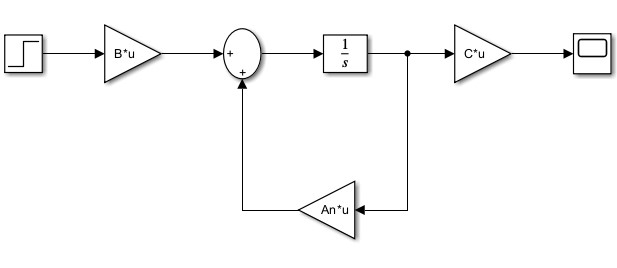
\includegraphics[width=\linewidth]{5.jpg}}
	\caption{Simulink}
	\label{fig5}
\end{figure}
\newpage
\section{Results}

\begin{figure}[htbp]
	\centerline{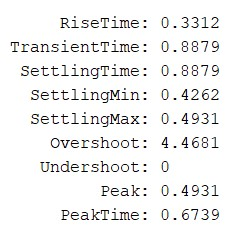
\includegraphics[width=0.5\linewidth]{3.jpg}}
	\caption{Step info after using controller}
	\label{fig3}
\end{figure}

\begin{figure}[htbp]
	\centerline{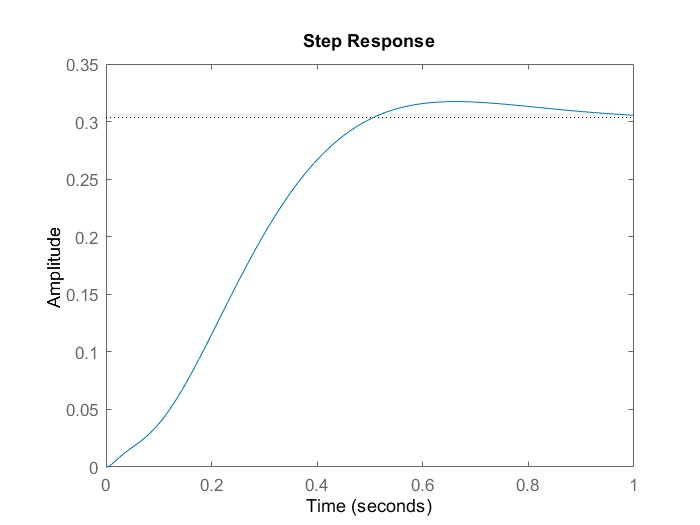
\includegraphics[width=\linewidth]{4.jpg}}
	\caption{Step response after using controller}
	\label{fig4}
\end{figure}

\section{Conclusion}
Using state feedback, we can precisely relocate the system’s poles, but it has some issues:
\begin{itemize}
	\item Permanently Disturbing the Steady-State Response: When we manipulate the poles, the steady-state response may be permanently affected.
	\item Inability to Use State Feedback: Despite its precision, state feedback cannot always be employed due to practical limitations.
	\item Saturation of the System: If the obtained coefficients exceed a certain limit, the system will saturate.
\end{itemize}
Based on the results, the overshoot was less than 5 percent, but the rising time was slightly more than the desired amount. This could be because an inaccurate formula was used.



\end{document}

